\section{Panorama} \label{sec:panorama}
%在我们深入讲解我们的系统之前,我们首先给出一个我们整个系统的全景图,如图1所示。这张全景图在一张图内尽可能详细的描述了我们尝试解决可什么问题以及如何解决了这个问题。

Before digging into the details of HyperPS, we first give a panorama view of our system, as depicted in Figure \ref{pic:panorama}. This panorama sketches in detail what problem we tried to solve and how we solve it.

%要在标题上对整个系统进行简单说明,既然是全景图,那么就应该包括如下的几点:要干什么,这个要最开始说,就一句话,说明我们要干什么,在这里就是如何在Hypervisor已经被危害的情况下如何保护guestVM的安全。这样就不需要说明威胁模型了,因为上面已经说了,是在Hypervisor已经被危害的前提下,就概括了图左边的内容;简要说明架构,这里要突出两个东西,一个是同层隔离,一个是将VMCS EPT移除到新的空间中。这个也是本文的两个最主要的东西,前者同层隔离提一句,要不要说好处呢?用修饰词把。后面VMCS,写效果,即VMCS移除以后会有什么效果,这个也是我们的最终的目的。
%HperPS利用内核页表构造一个与HostOS Hypervisor具有相同特权级的空间,并剥夺了原有内核对VMCS EPT的管理的特权,并将对应的特权赋予在隔离空间的Secure Code。
%HyperPS致力于在VMM HostOS已经被Compromised的前提下,剥离VMM直接管理VM的相关功能(VMM最重要的目的就是管理VM,现在将其最重要的功能剥离了,那么还要这个东西干啥用?)实现对保护VM的安全。
%TODO 修改,将HyperPS的Isolated 修改为separated
\begin{figure*}
    \centering
    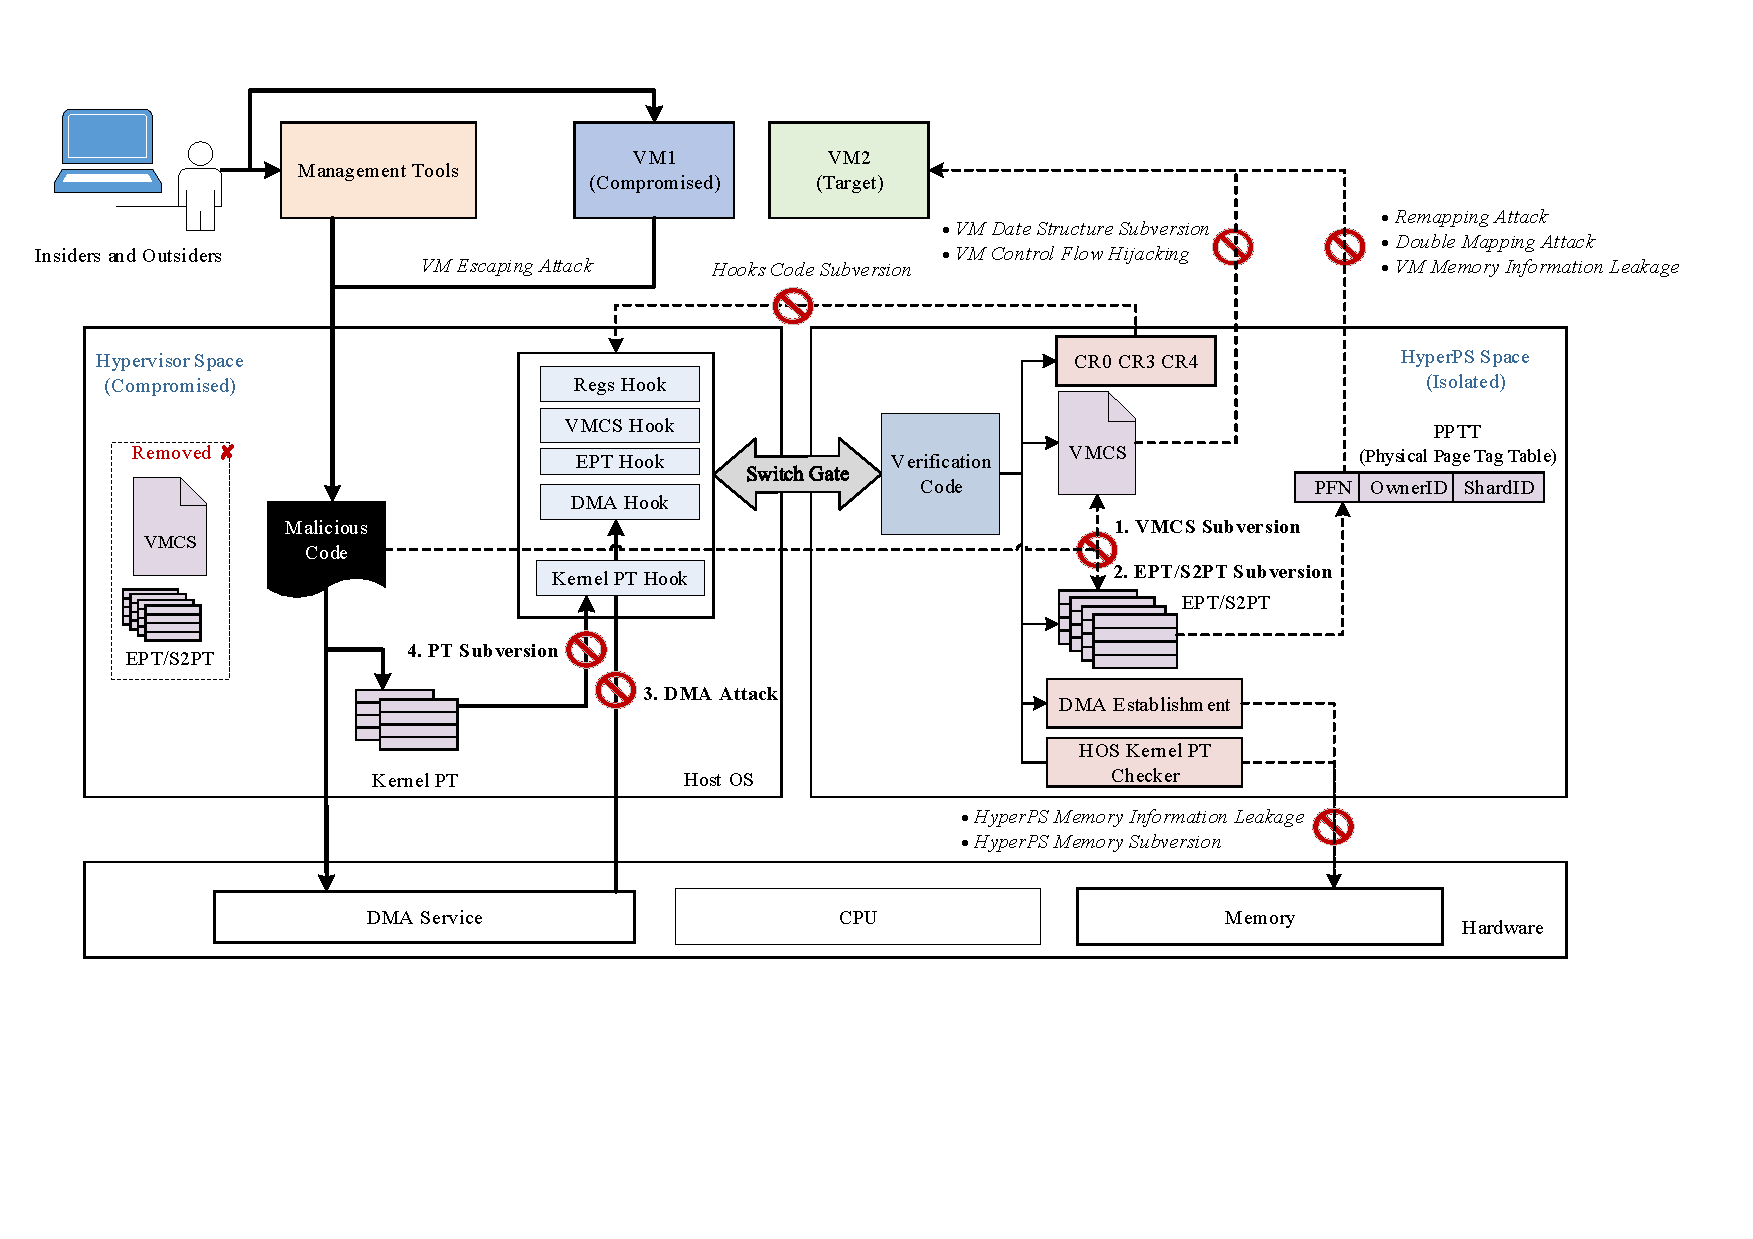
\includegraphics[width=1\textwidth]{IMG/panorama.pdf}
    \caption{The Panorama View of HyperPS. \\ HyperPS is committed to protect guest virtual machine under the compromised HostOS/Hypervisor. Privileges to manage VMCS and EPT are stripped from the compromised HostOS/Hypervisor into a separated and secure execution environment: HyperPS Space. The HyperPS space shares the same processor privilege as the HostOS. HyperPS does not rely on any special hardware or a higher privilege. Updates to VMCS and EPT are abandoned by the HyperPS, if the operations are not authorized or are adjudged as harmful to virtual machine.}
    \label{pic:panorama}
\end{figure*}

\subsection{Motivation} \label{sub:motivation}